\section*{k-Nearest Neighbor (k-NN)}


To analyze the performance of the InterCont method, it is essential to establish a baseline using recognized benchmark methods. 
Comparing a new proposal against established algorithms allows the scientific community to identify the specific conditions under which a method excels or fails. 
While contemporary research often evaluates a vast array of techniques—for instance, \citep{shenkar2022anomaly} compared InterCont against several state-of-the-art models—such an extensive comparison is beyond the scope of this thesis. 
Instead, I have selected two representative methods: one based on a statistical approach and the other on a distance-based approach.


This chapter is organized as follows:

\begin{itemize}
    \item k-Nearest Neighbor (k-NN): Introduced as a traditional distance-based approach for outlier detection.
    \item Minimum Covariance Determinant (MCD): Introduced as a traditional statistical method for robust estimation.
\end{itemize}

For each method, I will provide a literature review, define the underlying mechanics, and discuss their respective advantages and disadvantages alongside established solutions found in the literature.
\todo{this for the overall Methods Chapter?}


\section{k-Nearest Neighbor (k-NN)}
The $k$-Nearest Neighbor (k-NN) algorithm is a non-parametric method renowned for its simplicity and predictive accuracy \todo{add paper}. 
Initially detailed in a technical report for the US Air Force by \citet{fix1951discriminatory}, its formal theoretical proof was later established by \citet{1053964}.


The application of k-NN for outlier detection was pioneered by \citet{knox1998algorithms}. 
They defined an observation as an outlier if a specific fraction of the dataset lies beyond a predefined distance $D$, thereby introducing a distance-based hyperparameter. \todo{special hyperparameter?}
\citet{ramaswamy2000efficient} subsequently refined this approach by eliminating the distance threshold in favor of an internal outlier score, calculated based on the distances to an object's neighbors.
Under this framework, the $n$ points exhibiting the highest outlier scores are classified as anomalies, where $n$ is determined by a user-defined outlier ratio.


While the original InterCont publication does not explicitly specify the $k$-NN variant employed, the authors utilize the PyOD library \citep{zhao2019pyod}.
Given that PyOD implements the version proposed by \citet{ramaswamy2000efficient}, this specific iteration is utilized as the benchmark for this thesis.


The authors implemented an unsupervised learning approach. 
The algorithm executes the following procedure:

\begin{enumerate}
    \item The distances between $kth$ datapoints are calculated.
    \item The distances are ranked from highest to lowest.
    \item When the number of outliers $n$ \todo{whats the letter for outlier?} are known is known, the number of instaces $n$ with the highest distances are defined as outliers.
\end{enumerate}

k-NN is characterized as a "lazy learning" algorithm, meaning it does not construct an explicit generalization or internal model during a training phase. 
Consequently, the entire dataset must be retained. 
If a new instance is introduced, the algorithm must re-evaluate the proximity metrics across the dataset to determine its status.


To determine the $k$-nearest neighbors, the algorithm must quantify the proximity between a focal \todo{what?} instance and its neighboring data points. 
Various distance metrics can be employed to facilitate this calculation.
In traditional $k$-NN implementations, Euclidean distance is the standard metric.


It is defined as follows:


\begin{equation}
    d(p, q) = \sqrt{\sum_{i=1}^{n} (q_i - p_i)^2}
\end{equation}


However, the use of Euclidean distance renders $k$-NN non-affine equivariant. 
Because this metric treats all dimensions equally, variables with larger numerical ranges will dominate the distance calculation, potentially masking outliers that exist within the distribution of smaller-scaled variables.
This lack of equivariance implies that the model's outputs are sensitive to affine transformations. 
Consequently, the relative scaling of variables directly influences the identification of potential outliers.


To mitigate the effects of variable scaling, the dataset must be normalized. 
Min-Max Normalization is frequently employed to rescale all features to a fixed range, typically [0,1]. 

It is defined as follows:

\begin{equation}
    x_{norm} = \frac{x_i - x_{min}}{x_{max} - x_{min}}
\end{equation}

This technique performs a proportional transformation that preserves the original distributional and correlational structures. 
However, it is sensitive to extreme global outliers, which can compress the remaining data into a narrow, indistinguishable range.


Alternatively, Z-score normalization is utilized. 
This method transforms a variable such that the resulting distribution has a mean of $\mu=0$ and a standard deviation of $\sigma=1$. 

It is defined as follows:

\begin{equation}
    z = \frac{x_i - \mu}{\sigma}
\end{equation}

While effective for data approximating a Gaussian distribution, the utility of Z-score normalization diminishes if the data is heavily skewed or non-Gaussian, as the mean may not accurately represent the central tendency of the distribution \todo{review}.


The presence of extreme values often results in a distorted standard deviation $\sigma$, which complicates outlier detection due to the masking effect, where outliers inadvertently inflate the dispersion metrics used to identify them.
The Robust Scaler addresses this by substituting the mean $\mu$ and standard deviation $\sigma$ with more resilient statistics: the Median \todo{insert letter} and the Interquartile Range ($IQR$). 
By centering and scaling based on percentiles, the influence of anomalies on the transformation process is significantly reduced.

It is defined as follows:

\begin{equation}
    x_{robust} = \frac{x_i - \text{median}(X)}{\text{IQR}(X)}
\end{equation}

This method scales the data based on its internal distribution. 
By subtracting the median in the numerator, the data is centered such that the median corresponds to 0. 
Observations exceeding the median result in positive values, whereas those below it become negative.


The denominator facilitates the scaling process. 
By utilizing the $IQR$, the scaling factor is derived from a parameter that is inherently resistant to outliers. 
Consequently, the scaling maintains the relative distances between "normal" observations without the distortion typically introduced by extreme values in the dataset.


In addition to the outlier threshold, the parameter $k$ represents the primary hyperparameter of the algorithm. 
It defines the number of proximal observations utilized to compute the distance metrics.
An excessively low value for $k$ typically leads to overfitting, as the model becomes hyper-sensitive to local noise. 
This sensitivity often results in the identification of false positives and the generation of complex, fragmented decision boundaries. 
Conversely, while a larger $k$ provides a smoother decision surface and increased robustness to stochastic fluctuations, a value that is too high may lead to underfitting, where the model fails to detect local anomalies because they are overshadowed by the broader neighborhood.


Conversely, if $k$ is too large, the model becomes prone to underfitting. 
In this scenario, if an anomaly cluster contains fewer than $k$ observations, the algorithm incorporates points from more distant distributions into the distance calculation. 
This expansion skews the outlier scores and increases the likelihood of false negatives.
Consequently, the resulting decision boundaries become overly generalized, failing to capture critical local patterns within the data.
\todo{insert image}
\todo{rewrite text so image fits}


Selecting an optimal $k$ depends on the dataset's specific characteristics, including dimensionality, instance count, and the normalization technique applied. \todo{source}

Various methodologies exist for determining $k$. 
For instance, \citet{shenkar2022anomaly} employed a heuristic approach, manually setting the parameter to $k=5$. \todo{Is it GridSearch}
A more statistically rigorous method involves utilizing $k$-fold cross-validation to optimize the trade-off between bias and variance. 
This ensures that $k$ is tuned to the underlying data structure rather than selected arbitrarily.


Numerous variants of k-NN exist for anomaly detection. 
Utilizing the average distance across the neighborhood, rather than the absolute distance to the $k$-th neighbor, enhances the robustness and stability of detected outliers \citep{angiulli2002fast}. 
The literature proposes two primary \todo{really?} methodologies for computing the anomaly score: the distance to the specific $k$-th nearest neighbor or the mean distance to all $k$-nearest neighbors. 
By incorporating the average distance, the model mitigates the impact of local stochastic fluctuations, resulting in a more consistent scoring mechanism across diverse data distributions.
\todo{What are they solving?}
\todo{when can I use them as benchmarks}


In real-world applications, k-NN faces significant limitations because the true outlier ratio is frequently unknown, rendering any manual threshold selection arbitrary. 
Various k-NN derivatives attempt to mitigate this dependency. 
For example, Angle-Based Outlier Detection (ABOD) by \citet{kriegel2008angle} utilizes angular variance rather than spatial distances. 
Under this framework, an outlier is defined as a point where the variance of angles to other instances is substantially lower than that of inliers.
\todo{explain why I use plain k-nn as a benchmark method}


The $k$-NN algorithm offers several distinct advantages. 
Its outputs are inherently intuitive, facilitating straightforward interpretation of the detected anomalies.
While susceptible to the curse of dimensionality, the algorithm remains computationally efficient with large training sets.
Its reliance on distance metrics rather than complex optimization routines ensures a user-friendly implementation. 
As a non-parametric model, $k$-NN requires no prior assumptions regarding the underlying distribution of the dataset, providing the necessary flexibility to analyze complex data structures effectively.


The computational complexity of $k$-NN presents significant disadvantages in large-scale applications. 
As a memory-intensive approach, the model must store the entire dataset to facilitate predictions, which can result in substantial latency during the inference phase. \todo{inference phase? Defined it above if needed}
Furthermore, the reliance on distance-based metrics makes the algorithm susceptible to noise, which can negatively impact accuracy. 
Consequently, the selection of $k$ is critical to the model's performance, necessitating rigorous hyperparameter tuning to achieve an optimal balance between precision and robustness.

\begin{figure}[h] 
    \centering
    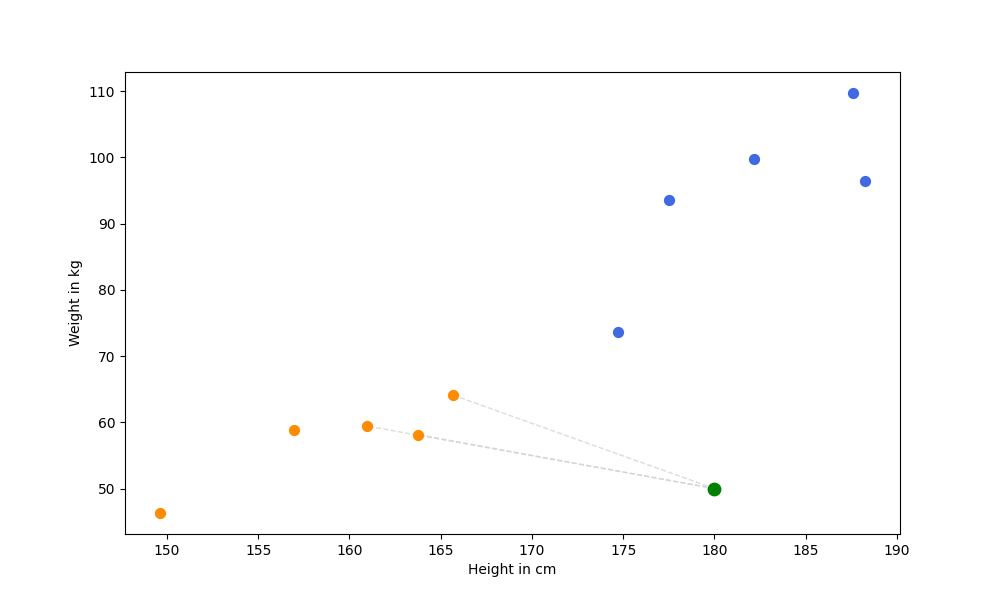
\includegraphics[width=1\linewidth]{Images/kNN/k-NN.png}
    \caption{grapfical depiction of $k$-NN algorithm}
    \label{fig:my_example}
\end{figure}